\section{Importazione dati nei Database}
\label{sec:database_ingestion}

Una volta completata la strutturazione dei documenti legali in formato JSON, si apre la fase di persistenza e indicizzazione dei dati. Nel contesto di questo progetto di tirocinio, l'architettura prevede il caricamento dei dati estratti all'interno del database a grafo Neo4j.

Per garantire la flessibilità e favorire un ambiente di sviluppo pulito e modulare, lo sviluppo del software ha visto l'applicazione del \textit{Repository Pattern} e l'uso di interfacce polimorfiche.

\subsection{I Modelli di Dominio}
\label{sec:modelli_dominio}
Prima di analizzare le strategie di persistenza, è fondamentale descrivere come i dati estratti vengano rappresentati. All'interno della cartella \texttt{models} di questo step, il sistema definisce le entità fondamentali del dominio normativo utilizzando il paradigma ad oggetti. Queste classi operano essenzialmente come \textit{Entities}: strutture dati pure, prive di logica di persistenza diretta o dipendenze verso i DBMS, il cui unico scopo è incapsulare i dati del dominio.

L'architettura dei modelli è rappresentata nel diagramma UML della Figura \ref{fig:domain-models-class-diagram}. Le principali classi sono:
\begin{itemize}
    \item \texttt{Entity}: Incapsula l'ente pubblico emittente, memorizzando i metadati di dominio.
    \item \texttt{LegalAct}: È la classe orchestratrice principale. Rappresenta l'atto legale nella sua interezza e contiene i metadati principali (title, publication\_date, file\_name) e soprattutto una lista \texttt{elements} che tiene traccia di tutti i sotto-elementi istanziati e delle loro relazioni gerarchiche.
    \item \texttt{StructuralElement}: È la classe base polimorfica per mappare le sottoclassi \texttt{Title}, \texttt{Chapter} e \texttt{Article}, mantenendo traccia del numero d'ordine e dell'eventuale rubrica.
    \item \texttt{Paragraph}: Rappresenta il comma ed è l'unità atomica d'informazione sulla quale verranno calcolati gli embedding.
\end{itemize}

\begin{figure}[H]
    \centering
    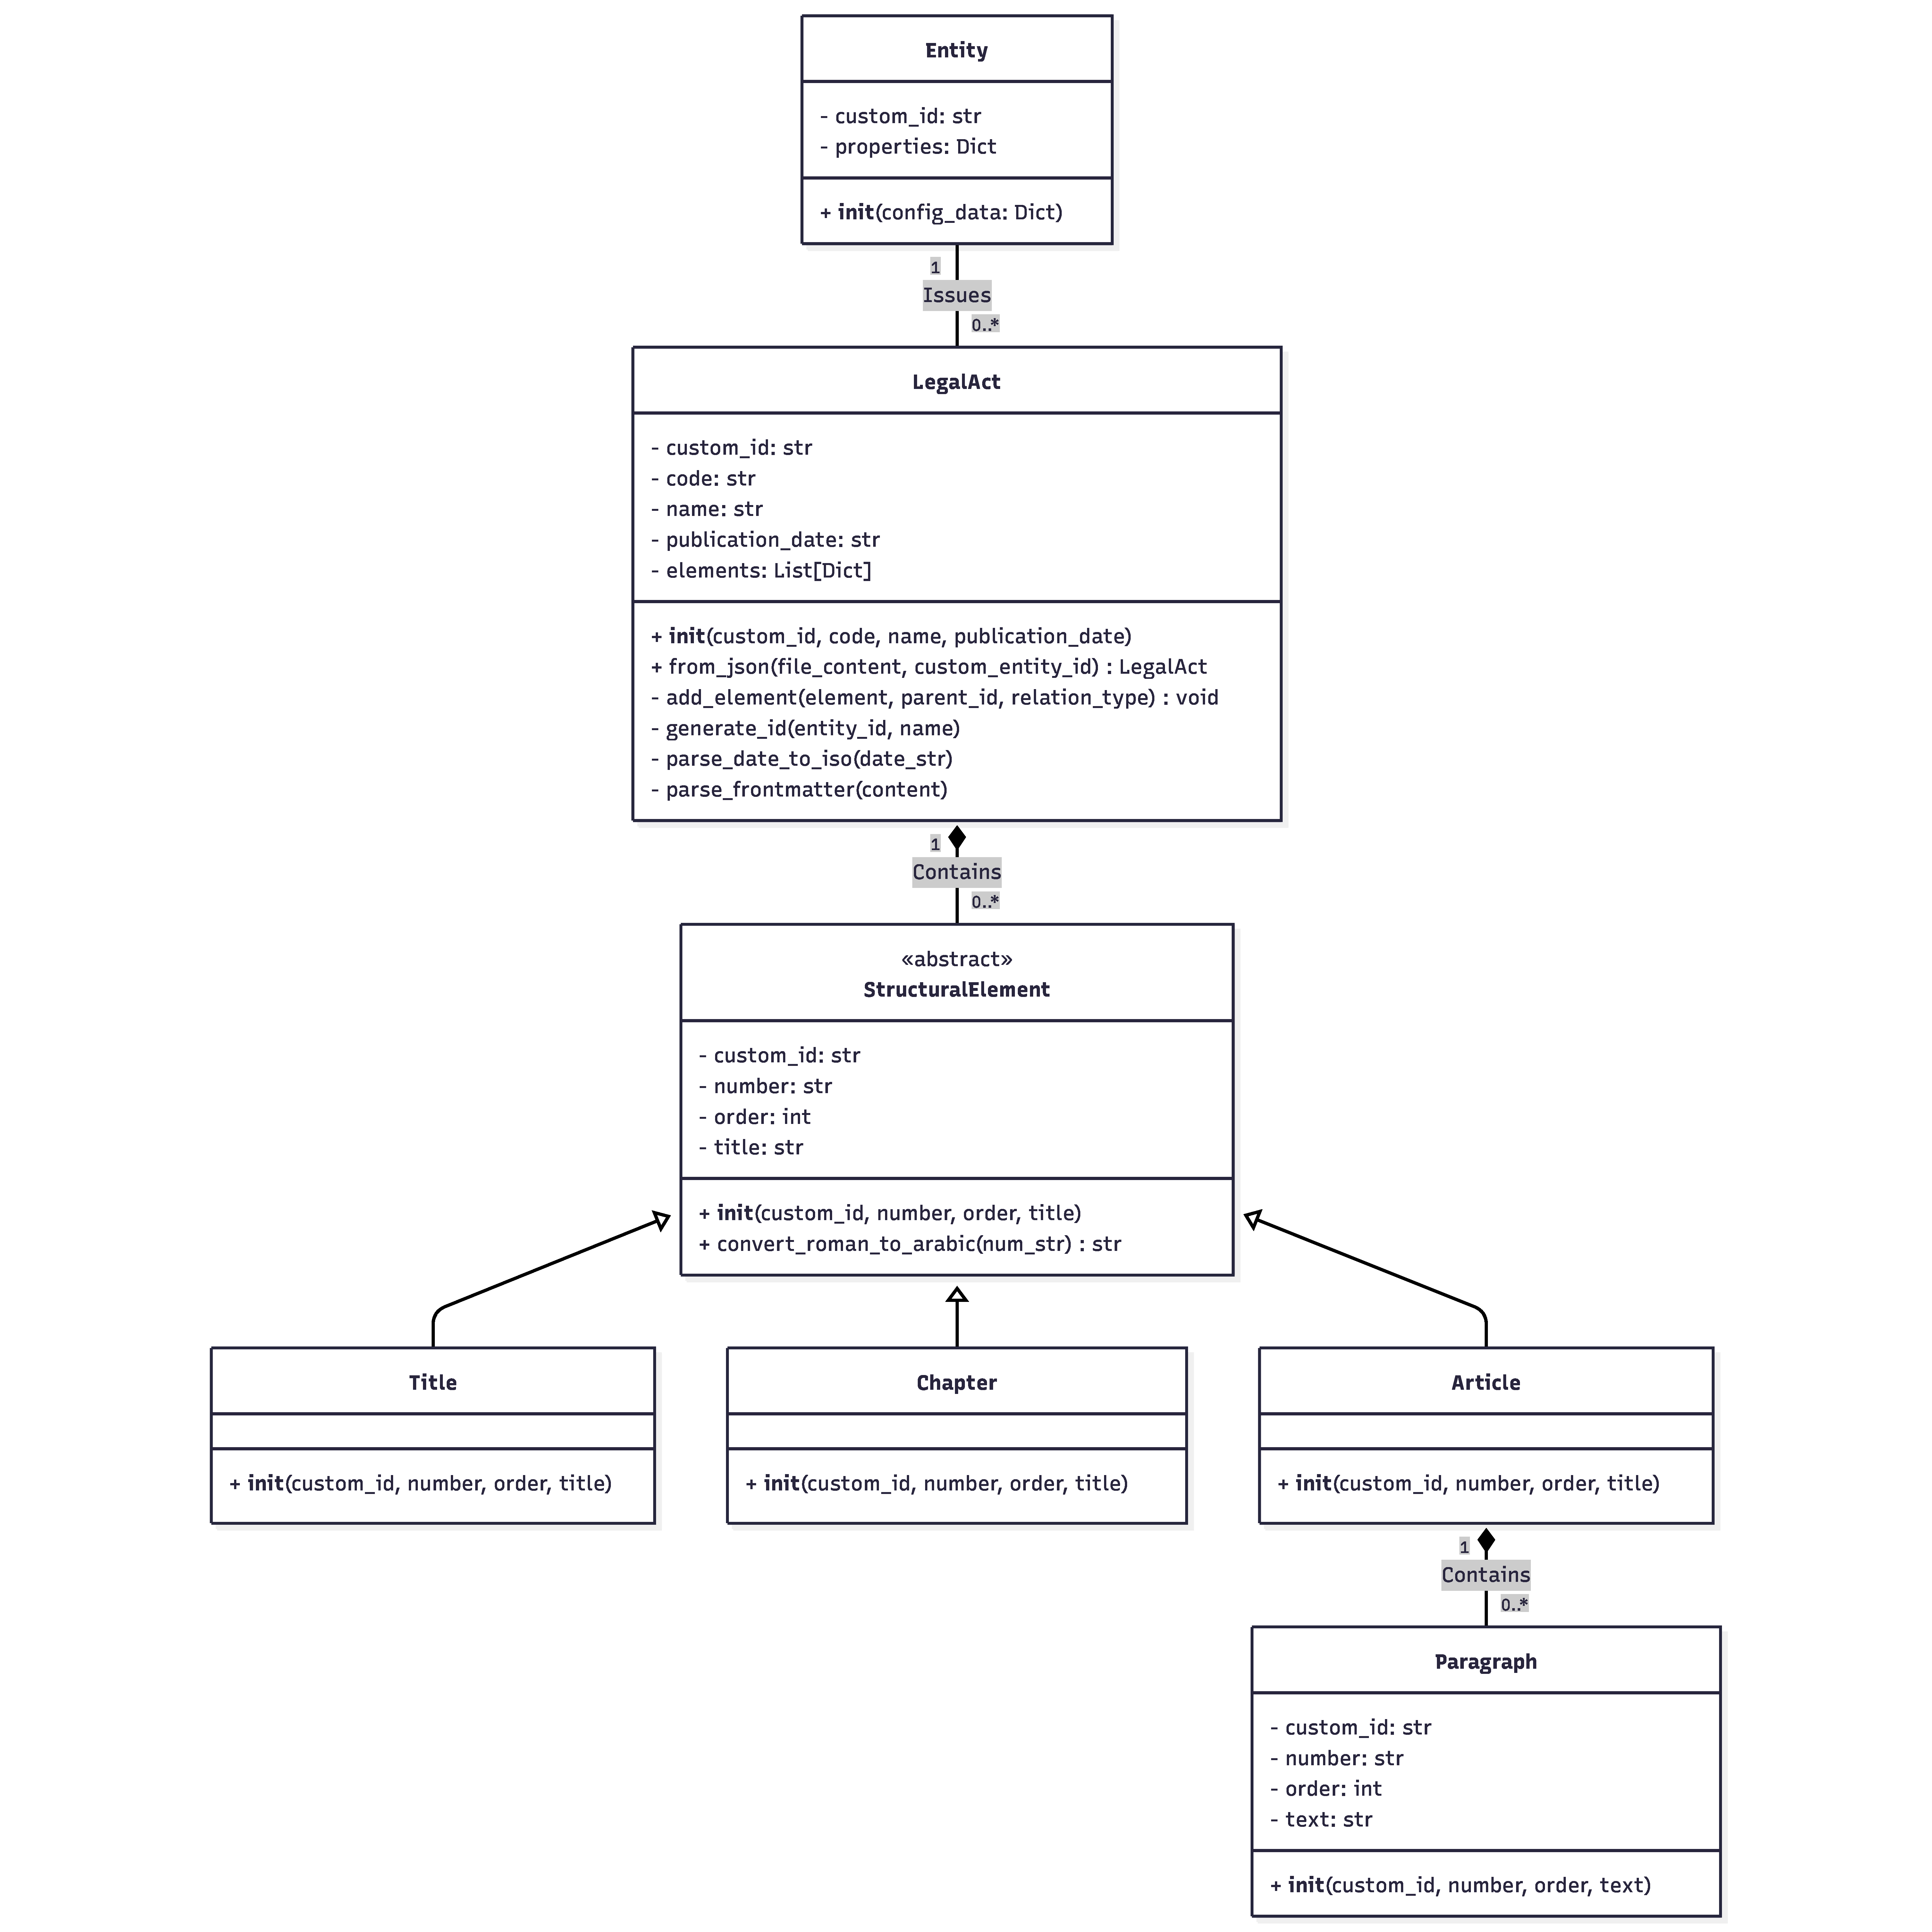
\includegraphics[width=1\textwidth]{_images/domain-models-class-diagram.pdf}
    \caption{Class Diagram dei modelli di dominio}
    \label{fig:domain-models-class-diagram}
\end{figure}


\subsection{Interfaccia per il disaccoppiamento della persistenza}
L'adozione di un'interfaccia comune di importazione nasce dalla precisa volontà di disaccoppiare la logica di lettura dei dati dalla loro effettiva persistenza fisica.
Sebbene l'attuale implementazione preveda l'utilizzo esclusivo del database a grafo Neo4j, questa scelta architetturale si rivela strategica per sviluppi futuri. Qualora si rendesse necessario integrare nuovi DBMS (ad esempio, un database puramente vettoriale dedicato esclusivamente agli embedding), sarà sufficiente implementare una nuova classe concreta senza dover alterare il flusso principale del programma. Inoltre, il disaccoppiamento garantisce un'elevata testabilità del codice, permettendo di validare la logica di dominio e il parsing dei documenti simulando le operazioni di salvataggio indipendentemente dal database sottostante.

Nel sistema sviluppato, l'interfaccia astratta di riferimento è rappresentata dalla classe \texttt{DBImporterInterface}. Essa definisce tre metodi fondamentali che ogni classe concreta deve implementare:
\begin{itemize}
    \item \texttt{connect()}: per la gestione e la validazione della connessione con l'istanza specifica del database;
    \item \texttt{import\_legal\_act(entity, legal\_act)}: per l'esecuzione effettiva di ingestion dell'atto normativo e dell'ente emittente;
    \item \texttt{close()}: per la chiusura sicura delle sessioni.
\end{itemize}


\subsection{Architettura del Database Neo4j}
\label{subsec:neo4j_architecture}

Il database modella fedelmente l'albero gerarchico discendente del documento, garantendo la flessibilità necessaria per gestire percorsi diretti qualora i livelli intermedi siano stati omessi durante la strutturazione JSON (es. \texttt{LegalAct $\rightarrow$ Article $\rightarrow$ Paragraph}). 

Le \textit{Label} dei nodi sul grafo (ovvero \textbf{Entity}, \textbf{LegalAct}, \textbf{Title}, \textbf{Chapter}, \textbf{Article} e \textbf{Paragraph}) riflettono rigorosamente la struttura delle classi di dominio già presentate nella Sezione \ref{sec:modelli_dominio}, così proprio come le \textit{Properties} dei nodi, che conservano i metadati principali e le informazioni testuali.

Un aspetto architetturale chiave, comune a tutti i nodi, è la presenza della proprietà \texttt{custom\_id}. Tale attributo codifica per intero il percorso gerarchico del nodo all'interno del documento (ad esempio, \texttt{ente\_\_atto\_\_title-1\_\_chapter-2\_\_article-3\_\_paragraph-4}). Grazie a questo approccio, il database può sfruttare l'indicizzazione su questa proprietà per individuare immediatamente un singolo nodo, azzerando le operazioni di attraversamento del grafo e garantendo un recupero delle informazioni in tempo costante.

All'interno di questa topologia, i nodi di tipo \textbf{Paragraph} ricoprono un ruolo centrale per le funzionalità avanzate del sistema. Oltre a conservare le proprietà testuali, in questi nodi vengono salvate le rappresentazioni vettoriali dei dati: in particolare, gli embedding semantici a dimensione variabile e un embedding strutturale a 128 dimensioni calcolato mediante l'algoritmo di \textit{Node2Vec} (maggiori informazioni sono nel capitolo \ref{sec:creazione_embedding}). L'archiviazione di tali vettori è progettata per abilitare le successive operazioni di interrogazione.

L'ecosistema di relazioni (\textit{Edges}) all'interno del grafo si articola in tre macro-categorie progettate per supportare le interrogazioni avanzate:
\begin{itemize}
    \item \textbf{Relazioni Strutturali}: Definiscono la topologia discendente del documento normativo. Comprendono l'arco \texttt{ISSUES} che lega l'Ente all'Atto, e la catena di contenimento gerarchico formata da \texttt{HAS\_TITLE}, \texttt{HAS\_CHAPTER}, \texttt{HAS\_ARTICLE} e \texttt{HAS\_PARAGRAPH}.
    \item \textbf{Relazioni Sequenziali}: I commi appartenenti allo stesso articolo sono concatenati linearmente tramite la relazione \texttt{NEXT\_PARAGRAPH}. Questa architettura a lista concatenata si rivela fondamentale per espandere dinamicamente la finestra di contesto durante la fase di interrogazione, permettendo di recuperare i commi logicamente antecedenti o successivi senza dover eseguire query computazionalmente costose per ricalcolare l'ordine strutturale.
    \item \textbf{Relazioni Legali}: Traducono in archi orientati sul grafo i collegamenti logici e giuridici intra-documento individuati dal prompt specializzato dell'LLM (Sezione \ref{sec:strutturazione_semantica}). Le cinque tipologie di relazione estratte vengono trasposte fedelmente nelle label \texttt{CITES}, \texttt{REPEALS}, \texttt{INTERPRETS}, \texttt{REPLACES} e \texttt{DEROGATES}. 
\end{itemize}

Occorre precisare che, sebbene lo schema dati supporti nativamente tutte le interazioni legali sopracitate, l'attuale popolamento del database non registra occorrenze per le relazioni \texttt{REPEALS} e \texttt{REPLACES}. Questa mancanza non è imputabile a un difetto del sistema di estrazione, bensì rappresenta un limite intrinseco dei documenti elaborati, che non contengono clausole esplicite di abrogazione o sostituzione strutturata.

\subsection{Dettagli Implementativi dell'Ingestion su Neo4j}
Un atto legale non può essere salvato tramite un'unica operazione atomica standard, a causa delle complesse connessioni tra i nodi, per questo motivo la responsabilità è stata distribuita su una serie di repository specializzati, ognuno deputato alla gestione del ciclo di vita di un singolo modello di dominio:
\begin{itemize}
    \item \texttt{EntityRepository}: Gestisce l'inserimento dei nodi relativi agli enti istituzionali.
    \item \texttt{LegalActRepository}: Inserisce il nodo radice dell'atto e lo ancora all'ente emittente.
    \item \texttt{StructuralElementRepository}: Incapsula la logica Cypher necessaria a creare i nodi intermedi del grafo e gli archi verso i rispettivi nodi padri.
    \item \texttt{ParagraphRepository}: Si occupa esclusivamente della persistenza dei nodi foglia contenenti il testo dei commi.
\end{itemize}

Per quanto riguarda il salvataggio delle relazioni trasversali, queste informazioni vengono lette da file JSON esterni dedicati (Sezione \ref{sec:estrazione_relazioni}), per poi essere elaborate da un metodo che, attraverso i \texttt{custom\_id} dei nodi salvati e indicizzati sul grafo, trova in maniera quasi istantanea i nodi correlati dall'estratto JSON ed esegue una query Cypher dedicata per la creazione dell'arco semantico.

\begin{lstlisting}[language=Cypher, caption={Query Cypher per l'inserimento delle relazioni legali}, label={lst:cypher_relationships}]
MATCH (s {custom_id: $source_id})
WITH s
MATCH (t {custom_id: $target_id})
MERGE (s)-[r:`<rel_type>`]->(t)
RETURN r
\end{lstlisting}

\noindent L'obiettivo di questa query è rintracciare i due nodi di interesse (sorgente e destinazione) tramite il loro identificativo univoco e stabilire una relazione orientata tra di essi.

Di seguito troviamo un esempio di relazione estratta in formato JSON, con ID parzialmente omessi per motivi di leggibilità:

\begin{lstlisting}[caption={Esempio reale di relazione estratta in formato JSON}, label={lst:json-cites}, breaklines=true]
{
  "sourceId": "ente-provincia-taranto__contratto-collettivo-[...]__title-2__chapter-2__article-8__paragraph-6",
  "relationshipType": "CITES",
  "targetId": "ente-provincia-taranto__contratto-collettivo-[...]__title-2__chapter-2__article-8__paragraph-1"
}
\end{lstlisting}

A supporto di quanto descritto, la Figura \ref{fig:relationship_example} fornisce una rappresentazione visiva delle relazioni instaurate tra i nodi dell'articolo 8 del seguente atto: \texttt{"CCNL del personale non dirigente del comparto regioni e autonomie locali"}

\begin{figure}[H]
    \centering
    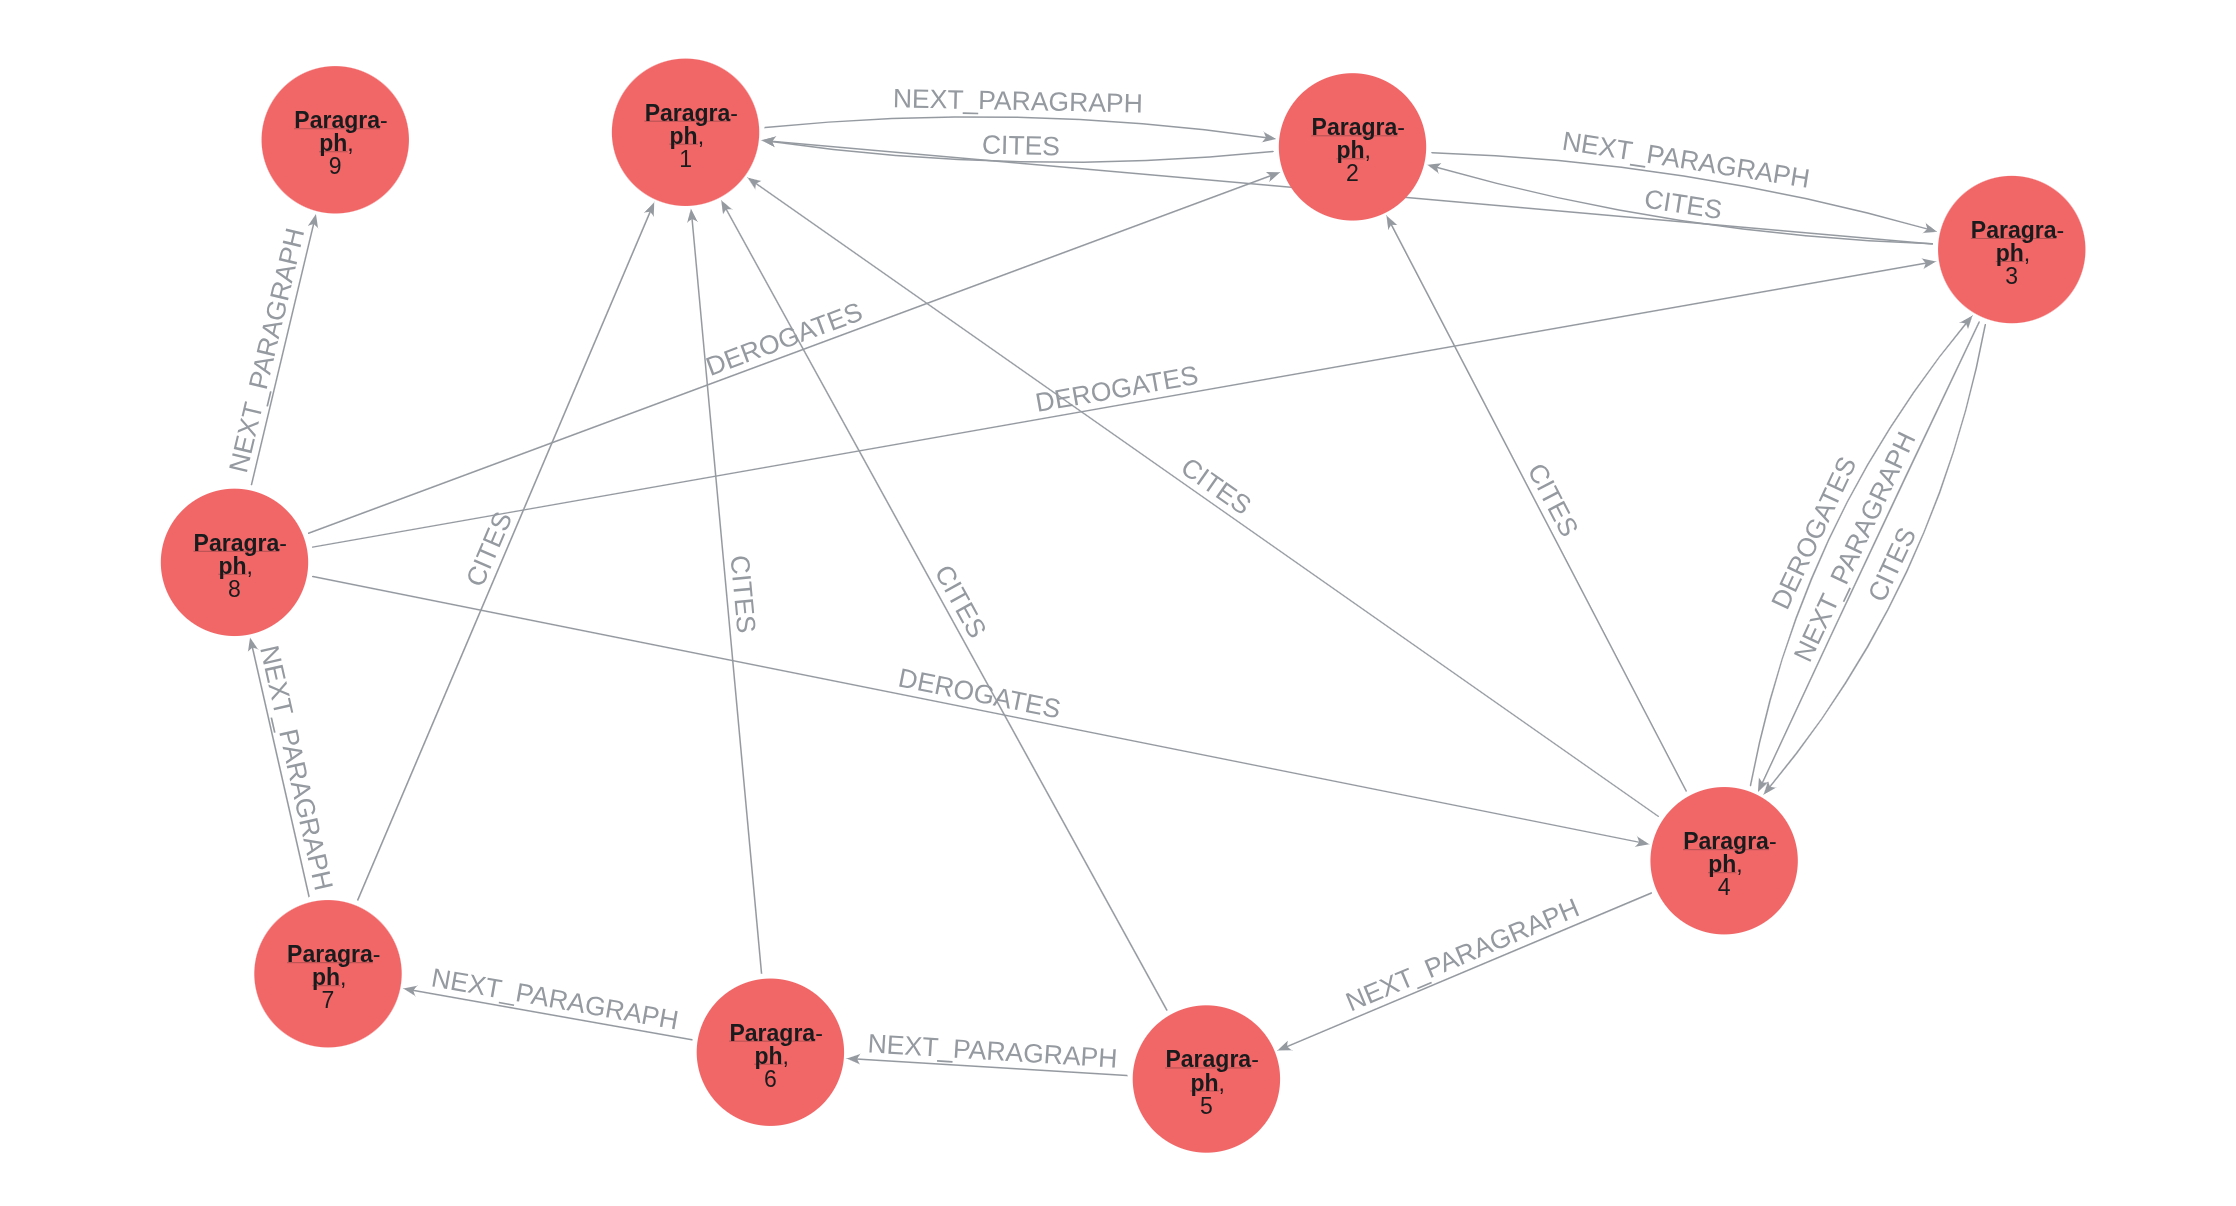
\includegraphics[width=1\textwidth]{_images/relationship.png}
    \caption{Rappresentazione visiva delle relazioni instaurate tra i nodi dell'articolo 8 di un atto normativo.}    
    \label{fig:relationship_example}
\end{figure}

\subsection{Risultati e Metriche}
L'esecuzione della pipeline di ingestion ha dimostrato un'elevata efficienza, completando il caricamento dell'intero dataset all'interno del database in un tempo complessivo di \textbf{50.29 secondi}.

Il processo ha popolato il grafo con un totale di 8.535 nodi e 14.201 relazioni. Di seguito viene riportato il dettaglio quantitativo delle entità di dominio e degli archi salvati.

La Tabella \ref{tab:statistiche_nodi} illustra la distribuzione dei nodi all'interno del grafo, raggruppati per \textit{Label}. Come si può osservare dai dati, vi è una netta preponderanza numerica dei nodi \texttt{Paragraph}, i quali rappresentano l'unità atomica d'informazione su cui si basano le successive operazioni di embedding e ricerca.

\begin{table}[H]
    \centering
    \renewcommand{\arraystretch}{1.2}
    \begin{tabular}{|l|r|}
        \hline
        \textbf{Label Nodo} & \textbf{Quantità} \\
        \hline
        \texttt{Paragraph} & 6.396 \\
        \texttt{Article} & 1.802 \\
        \texttt{Chapter} & 147 \\
        \texttt{LegalAct} & 95 \\
        \texttt{Title} & 93 \\
        \texttt{Entity} & 2 \\
        \hline
    \end{tabular}
    \caption{Statistica dei nodi inseriti nel database Neo4j.}
    \label{tab:statistiche_nodi}
\end{table}

Per quanto riguarda invece le interconnessioni tra le entità, la Tabella \ref{tab:statistiche_relazioni} dettaglia il conteggio esatto degli archi strutturali, sequenziali e legali creati durante l'importazione.

\begin{table}[H]
    \centering
    \renewcommand{\arraystretch}{1.2}
    \begin{tabular}{|l|r|}
        \hline
        \textbf{Tipo di Relazione} & \textbf{Quantità} \\
        \hline
        \texttt{HAS\_PARAGRAPH} & 6.396 \\
        \texttt{NEXT\_PARAGRAPH} & 4.594 \\
        \texttt{HAS\_ARTICLE} & 1.802 \\
        \texttt{CITES} & 1.030 \\
        \texttt{HAS\_CHAPTER} & 147 \\
        \texttt{ISSUES} & 95 \\
        \texttt{HAS\_TITLE} & 93 \\
        \texttt{DEROGATES} & 41 \\
        \texttt{INTERPRETS} & 3 \\
        \hline
    \end{tabular}
    \caption{Statistica delle relazioni inserite nel database Neo4j.}
    \label{tab:statistiche_relazioni}
\end{table}

Come si evince dalla Tabella \ref{tab:statistiche_relazioni}, l'analisi degli archi conferma la solidità dell'architettura a lista concatenata, evidenziata dal notevole volume di relazioni \texttt{NEXT\_PARAGRAPH} (4.594), essenziali per l'espansione dinamica del contesto in fase di retrieval. 

Inoltre, analizzando sempre i medesimi dati in merito agli archi logico-legali, si osserva una netta predominanza delle relazioni di citazione (\texttt{CITES}, 1.030 occorrenze), seguite da un numero minoritario di deroghe (\texttt{DEROGATES}, 41) e interpretazioni (\texttt{INTERPRETS}, 3). Coerentemente con quanto anticipato nella Sezione \ref{subsec:neo4j_architecture}, le metriche riportate confermano l'assenza totale di occorrenze per le relazioni di abrogazione (\texttt{REPEALS}) e sostituzione (\texttt{REPLACES}) all'interno di questo specifico bacino documentale.

\subsection{Visualizzazione del Grafo}
A conclusione di questo capitolo, si propone una rappresentazione visiva di un estratto del database Neo4j volta a mostrare in maniera intuitiva la topologia della rete. Nella Figura \ref{fig:graph-visualization} è possibile osservare la struttura gerarchica e le connessioni tra le diverse entità, evidenziate mediante una differenziazione cromatica:
\begin{itemize}
    \item I \textbf{nodi gialli} rappresentano l'ente emittente (\texttt{Entity});
    \item I \textbf{nodi azzurri} indicano gli atti legali (\texttt{LegalAct});
    \item I \textbf{nodi rossi} corrispondono ai commi (\texttt{Paragraph});
    \item I \textbf{restanti nodi} raffigurano le altre parti della gerarchia strutturale del documento, ossia i titoli (\texttt{Title}), i capi (\texttt{Chapter}) e gli articoli (\texttt{Article}).
\end{itemize}

\begin{figure}[H]
    \centering
    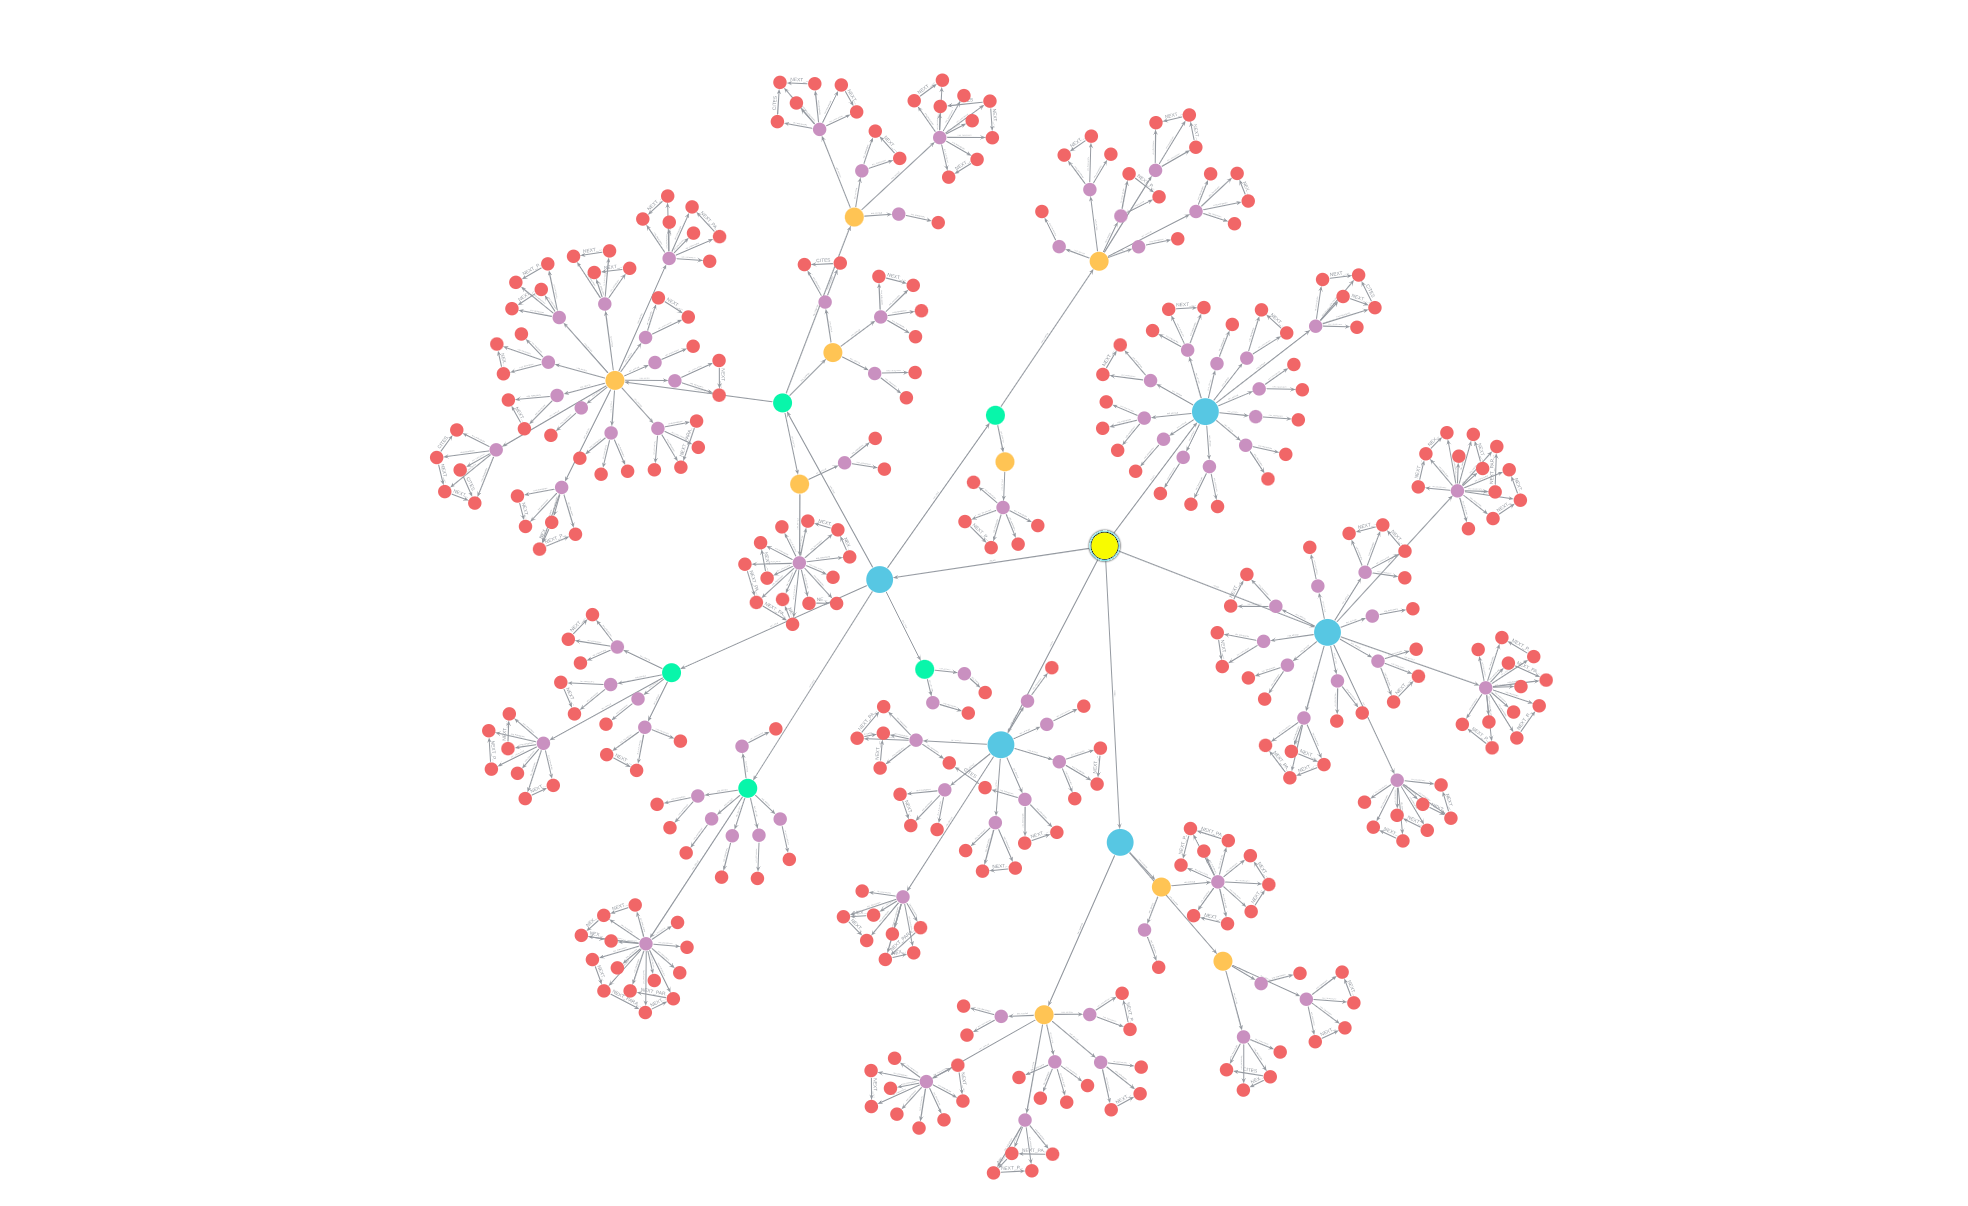
\includegraphics[width=1\textwidth]{_images/graph-visualization.png}
    \caption{Rappresentazione visiva di un estratto del database a grafo Neo4j.}
    \label{fig:graph-visualization}
\end{figure}